\documentclass[a4paper,12pt]{article} % тип документа

%  Русский язык
\usepackage[T2A]{fontenc}			% кодировка
\usepackage[utf8]{inputenc}			% кодировка исходного текста
\usepackage[english,russian]{babel}	% локализация и переносы

\usepackage{graphicx}               % импорт изображений
\usepackage{wrapfig}                % обтекаемые изображения
\graphicspath{{pictures/}}          % обращение к подкаталогу с изображениями
\usepackage[14pt]{extsizes}         % для того чтобы задать нестандартный 14-ый размер шрифта
\usepackage[warn]{mathtext}         % русский язык в формулах
\usepackage{indentfirst}            % indent first
\usepackage[margin = 25mm]{geometry}% отступы полей
\usepackage[table,xcdraw]{xcolor}   % таблицы
\usepackage{amsmath,amsfonts,amssymb,amsthm,mathtools} % Математика
\usepackage{wasysym}                % ???
\usepackage{upgreek}                % ???  
\usepackage{caption}
\captionsetup{labelsep = period}
\usepackage{mathrsfs}
\usepackage{makecell}
\usepackage{gensymb} % degree symbol



\pagestyle{empty}


\begin{document}
	
\section*{Билет №5.}

\subsection*{Необходимые определения и предложения билета}
\noindent \textbf{Определение:} множество $Q = [a_1, b_1) \times [a_2, b_2) \times \dots \times [a_m, b_m)$ будем называть клеткой в $\mathbb{E}^m$.

\vspace{3mm}

\noindent \textbf{Определение:} множество $G \subset \mathbb{E}^m$ будем называть клеточным, если оно является объединением \textbf{конечного} числа попарно непересекающихся клеток:
\begin{equation*}
	G = \bigcup_{j = 1}^k Q_j, \hspace{10mm} Q_i \cap Q_j = \varnothing, \text{ }i \neq j.
\end{equation*}


\begin{figure}[h!]
	\begin{minipage}[h]{0.49\linewidth}
		\center{\includegraphics[scale = 0.5]{G(Клет).jpg} \\ G - клеточное множество}
	\end{minipage}
	\hfill
	\begin{minipage}[h]{0.49\linewidth}
		\center{\includegraphics[scale = 0.5]{G(Неклет).jpg} \\ G - не клеточное множество}
	\end{minipage}
\end{figure}

\noindent \textbf{Свойства клеточных множеств:}

$\textbf{1}^\circ$ Объединение \textbf{конечного} числа попарно непересекающихся клеточных множеств есть клеточное множество.

\noindent \textbf{Доказательство:}

$G$ и $H$ - клеточные множества. Тогда:
\begin{equation*}
	G = \bigcup_{j = 1}^k Q_j, \hspace{20mm} H = \bigcup_{j = k + 1}^n Q_j.
\end{equation*}

Значит:
\begin{equation*}
	G \cup H = \bigcup_{j = 1}^n Q_j - \text{клеточное множество}.
\end{equation*}

$\textbf{2}^\circ$ Пересечение двух клеток есть клетка.

\noindent \textbf{Доказательство:} 

Пусть $Q_1 = [a_1, b_1) \times [a_2, b_2) \times \dots \times [a_m, b_m)$, а $Q_2 = [c_1, d_1) \times [c_2, d_2) \times \dots \times [c_m, d_m)$. Тогда возможны два случая:

а) $\exists j$: $[a_j, b_j) \cap [c_j, d_j) = \varnothing \Rightarrow Q_1 \cap Q_2 = \varnothing $ - клетка;

б) $\forall j \longmapsto [a_j, b_j) \cap [c_j, d_j) = [e_j, f_j) \Rightarrow Q_1 \cap Q_2 = [e_1, f_1) \times [e_2, f_2) \times \ldots \times [e_m, f_m)$ - клетка.

\vspace{5mm}

$\textbf{3}^\circ$ Пересечение двух клеточных множеств есть клеточное множество.

\noindent \textbf{Доказательство:}

Пусть $G_1$ и $G_2$ - клеточные множества.

$G_1 = Q_1^1 \cup Q_2^1 \cup \ldots \cup Q_k^1$

$G_2 = Q_1^2 \cup Q_2^2 \cup \ldots \cup Q_n^2$

Обозначим $Q_{ij} = Q_i^1 \cap Q_j^2, \text{ } i = \overline{1, k}, \text{ } j = \overline{1, n}.$

$Q_{ij}$ - клетка (свойство $\textbf{2}^\circ$).

$G_1 \cap G_2 = \bigcup\limits_{i, j} Q_{ij} = \bigcup\limits_{i = 1}^k \bigcup\limits_{j = 1}^n Q_{ij}$ - объединение попарно непересекающихся клеток есть клеточное множество.

\vspace{5mm}

$\textbf{4}^\circ$ Разность двух клеток есть клеточное множество.

\noindent \textbf{Доказательство:}

$Q_1$ и $Q_2$ - клетки. $Q = Q_1 \cap Q_2$ - клетка (свойство $\textbf{2}^\circ$). Тогда

$Q_1 \backslash Q_2 = Q_1 \backslash Q$.

Существует такое разбиение клетки $Q_1$ на более мелкие клетки, что $Q$ является одной из них $\Rightarrow$

$\Rightarrow Q_1 \backslash Q_2$ - клеточное множество.

\begin{figure}[h!]
	\centering
	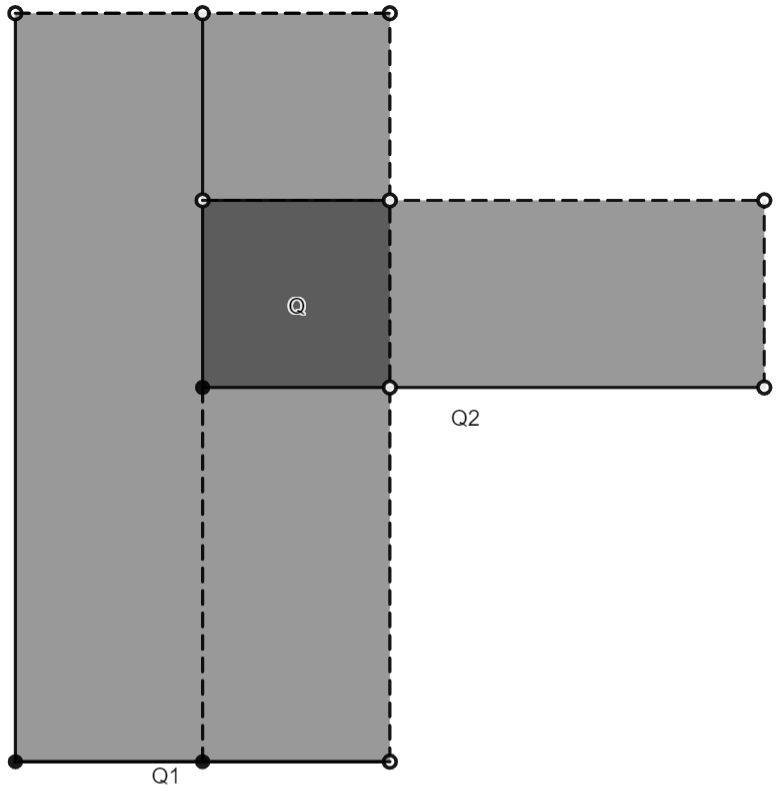
\includegraphics[scale=0.57]{Q.jpg}
\end{figure} 



$\textbf{5}^\circ$ Разность двух клеточных множеств есть клеточное множество.

\noindent \textbf{Доказательство:}

\begin{equation*}
	G_1 = \bigcup_{j = 1}^k Q_j^1, \hspace{20mm} G_2 = \bigcup_{j = 1}^n Q_j^2.
\end{equation*}


\begin{equation*}
	G_1 \backslash Q_1^2 = \bigcup_{i = 1}^k \left(Q_i^1 \backslash Q_1^2\right) = \bigcup_{i = 1}^k G_{i1} 
\end{equation*}


$G_{i1}$ - клеточное множество (свойство $\textbf{4}^\circ$).

$G_{i1} \cap G_{j1} = \varnothing$, если $i \neq j \Rightarrow$

$\Rightarrow G_1 \backslash Q_1^2$ - клеточное множество (свойство $\textbf{1}^\circ$).

\begin{equation*}
	G_1 \backslash G_2 = G_1 \backslash \left( \bigcup_{j = 1}^n Q_j^2\right) = \bigcap_{j = 1}^n\left(G_1 \backslash Q_j^2\right) = \bigcap_{j = 1}^n\left(\bigcup_{i = 1}^k G_{ij}\right)
\end{equation*}

Последнее является клеточным множеством, так как $G_{ij} \cap G_{sl} = \varnothing$, если $i \neq s$ или $j \neq l$. Откуда получаем, что $G_1 \backslash G_2$ - клеточное множество.

\vspace{5mm}

$\textbf{6}^\circ$ Объединение \textbf{конечного} числа клеточных множеств есть клеточное множество.

\noindent \textbf{Доказательство:}

1) $G_1$ и $G_2$.

$G_1 \cup G_2 = \left(G_1 \backslash G_2\right) \cup \left(G_2 \backslash G_1\right) \cup \left(G_1 \cap G_2\right)$;

Последние три скобки являются попарно непересекающимися клеточными множествами $\stackrel{\textbf{1}^\circ}{\Rightarrow}$ $G_1 \cup G_2$ - клеточное множество.

2) Далее для $G_3, G_4, \ldots, G_n$ по индукции.

\vspace{7mm}

\textbf{Таким образом, объединение, пересечение и разность конечного числа клеточных множеств есть клеточное множество.}

\vspace{7mm}

\noindent \textbf{Определение:} мерой клетки $Q$ назовем число:

$m(Q) = (b_1 - a_1)\cdot (b_2 - a_2)\cdot\ldots\cdot (b_m - a_m)$;

$m(\varnothing) = 0$.


\noindent \textbf{Определение:} мерой клеточного множества $G$ назовем число:
\begin{equation*}
	m(G) = \sum_{j = 1}^{k} m(Q_j); \hspace{20mm} m(\varnothing) = 0.
\end{equation*}


\noindent \textbf{Лемма:} мера клеточного множества $G$ не зависит от способа разбиения этого множества на клетки.

\noindent \textbf{Доказательство:}

Пусть $G = Q_1 \cup Q_2 \cup \ldots \cup Q_k$ и также $G = Q'_1 \cup Q'_2 \cup \ldots \cup Q'_n$. Тогда обозначим $Q_{ij} = Q_i \cup Q'_j, \text{ } i = \overline{1, k}, \text{ } j = \overline{1, n}.$

Понятно, что 
\begin{equation*}
	Q_i = \bigcup_{j = 1}^n Q_{ij}, \hspace{20mm} Q'_j = \bigcup_{j = 1}^k Q_{ij}.
\end{equation*}

Тогда:

\begin{equation*}
	m(G) =  \sum_{i = 1}^{k} m(Q_i) = \sum_{i = 1}^{k} \sum_{j = 1}^{n} m(Q_{ij}) = \sum_{j = 1}^{n} \sum_{i = 1}^{k} m(Q_{ij}) = \sum_{j = 1}^{n} m(Q'_j) = m(G).
\end{equation*}

\noindent \textbf{Предложение 1:} если клеточные множества $G_1, G_2, \ldots, G_n$ попарно не пересекаются, то для $G = \bigcup\limits_{j = 1}^n G_j$ выполняется $m(G) = \sum\limits_{j = 1}^n m(G_j)$.

\noindent \textbf{Доказательство:}

$G_j = \bigcup\limits_{i = 1}^{k_j} Q_i^j, \text{ } j = \overline{1, n}.$

Тогда

$G = \bigcup\limits_{j = 1}^n G_j = \bigcup\limits_{j = 1}^n \bigcup\limits_{i = 1}^{k_j} Q_i^j = \bigcup\limits_{\substack{1 \leqslant j \leqslant n,\\ 1\leqslant i \leqslant k_j}} Q_i^j$

Все клетки из последнего объединения попарно не пересекаются, поэтому:

$m(G) = \sum\limits_{\substack{1 \leqslant j \leqslant n,\\ 1\leqslant i \leqslant k_j}} m(Q_i^j) = \sum\limits_{j = 1}^n m(G_j)$.

\vspace{5mm}

\noindent \textbf{Предложение 2:} если $G_1$ и $G_2$ - клеточные множества и $G_1 \subset G_2$, то $m(G_2) = m(G_1) + m(G_2 \backslash G_1)$,  $m(G_1) \leqslant m(G_2)$.

\noindent \textbf{Доказательство:}

$G_2 = G_1 \cup (G_2 \backslash G_1) = G_1 \cup G$.

$G_1 \cap G = \varnothing \stackrel{\text{пр.1}}{\Longrightarrow} m(G_2) = m(G_1) + m(G_2 \backslash G_1) \Rightarrow m(G_1) \leqslant m(G_2)$.


\noindent \textbf{Предложение 3:} если $G_1, G_2, \ldots, G_k$ - клеточные множества, $G = \bigcup\limits_{j = 1}^k G_j$, то $m(G) \leqslant \sum\limits_{j = 1}^k m(G_j)$.

\noindent \textbf{Доказательство:}

Для $G_1$ и $G_2$ по предложению 2, а далее по индукции.

\vspace{3mm}

\noindent \textbf{Предложение 4:} для любого клеточного множества $G$ и $\forall \varepsilon > 0$ $\exists G_{\varepsilon}, G^{\varepsilon}$ - клеточные множества такие, что:

1) $G_{\varepsilon} \subset \overline{G_{\varepsilon}} \subset \text{int } G \subset G$;\hspace{8mm} $m(G) - m(G_{\varepsilon}) < \varepsilon$;

2) $G \subset \overline{G} \subset \text{int } G^{\varepsilon} \subset G^{\varepsilon}$; \hspace{7mm} $m(G^{\varepsilon}) - m(G) < \varepsilon$.

\noindent \textbf{Доказательство:}

1) $G = Q_1 \cup Q_2 \cup \ldots \cup Q_k$.

Рассмотрим отдельную клетку $Q = [a_1, b_1) \times [a_2, b_2) \times \ldots \times [a_m, b_m)$

\begin{figure}[h!]
	\centering
	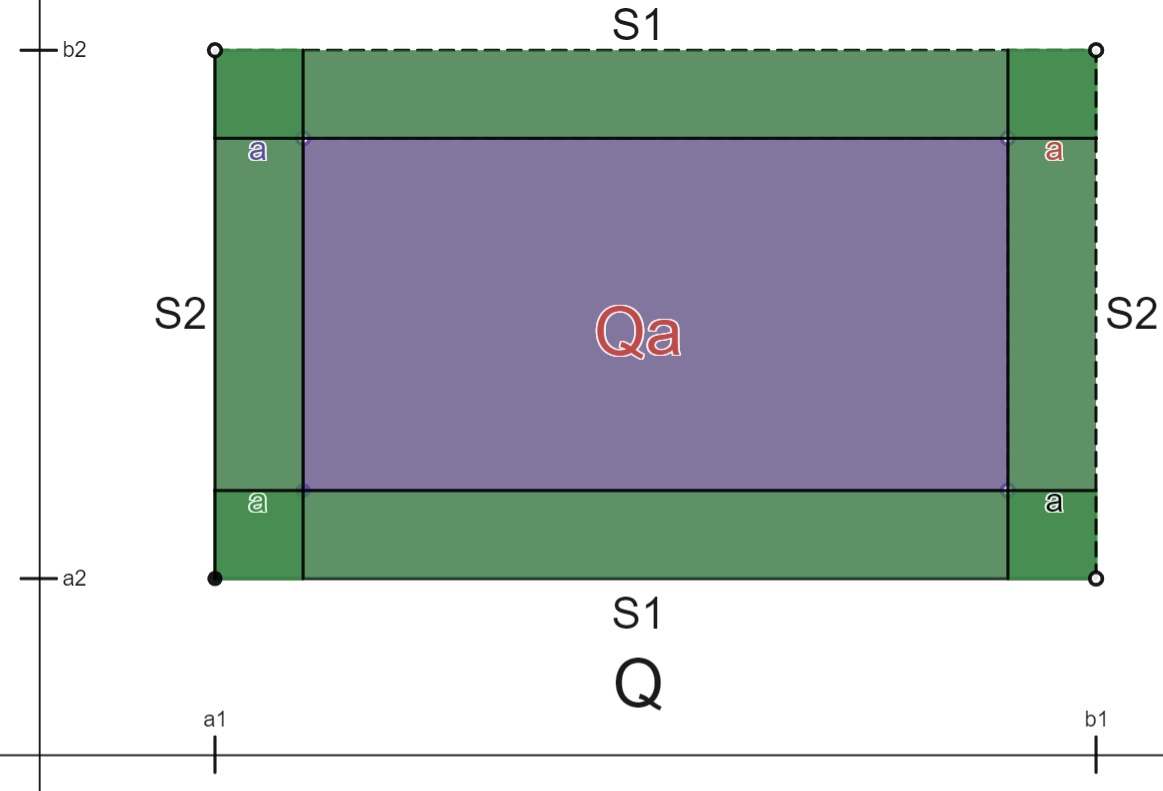
\includegraphics[scale=0.6]{Пред4.jpg}
	\caption*{Случай при $m$ = 2}
\end{figure}

$m(Q_a) = \prod\limits_{j = 1}^m (b_j - a_j - 2a)$, $Q_a \subset Q$.

$S_j = \prod\limits_{\substack{i = 1,\\ i \neq j}}^m (b_j - a_j)$;

Тогда 

$m(Q) < m(Q_a) + 2a\cdot\sum\limits_{j = 1}^m S_j = m(Q_a) + 2aS \Rightarrow m(Q) - m(Q_a) < 2aS = \varepsilon$.

Тогда для одной клетки $a = \frac{\varepsilon}{2S}$.

Так как $G = Q_1 \cup Q_2 \cup \ldots \cup Q_k$, то $a = \frac{\varepsilon}{2Sk}$.

Получаем $G_{\varepsilon} = \bigcup\limits_{i = 1}^k (Q_a)_i$.

Таким образом, $G_{\varepsilon} \subset \overline{G_{\varepsilon}} \subset \text{int } G \subset G$.

\vspace{3mm}
2) Доказывается аналогично 1).





\subsection*{Определение измеримости по Жордану множества в $m$-мерном евклидовом пространстве.}
\noindent \textbf{Определение:} множество $X \subset \mathbb{E}^m$ называется измеримым по Жордану, если $\forall \varepsilon > 0 \text{ }\exists G_{\varepsilon}$ и $G^{\varepsilon}$ - клеточные множества такие, что $G_{\varepsilon} \subset X \subset G^{\varepsilon}$ и $m(G^{\varepsilon}) - m(G_{\varepsilon}) < \varepsilon$. 

\vspace{3mm}

\noindent \textbf{Определение:} мерой измеримого по Жордану множества $X \subset \mathbb{E}^m$ называется такое число $m(X)$, что $\forall G_{\varepsilon},\text{ } G^{\varepsilon}$ таких, что $G_{\varepsilon} \subset X \subset G^{\varepsilon} \longmapsto m(G_{\varepsilon}) \leqslant m(X) \leqslant m(G^{\varepsilon})$.

\vspace{3mm}

\noindent \textbf{Лемма:} для любого измеримого по Жордану множества $X$ его мера $m(X)$ существует и единственна, причем

\begin{equation*}
	m(X) = \overline{m}(X) = \underline{m}(X),
\end{equation*}

\noindent где $\overline{m}(X) = \inf\limits_{X \subset G^{\varepsilon}} m(G^{\varepsilon})$ - верхняя (внешняя) мера $X$;

\noindent $\underline{m}(X) = \sup\limits_{X \subset G_{\varepsilon}} m(G_{\varepsilon})$ - нижняя (внутренняя) мера $X$.

\noindent \textbf{Доказательство:} 

Так как $G_{\varepsilon} \subset X \subset G^{\varepsilon}$, то $m(G_{\varepsilon}) \leqslant m(G^{\varepsilon}) \Rightarrow$ $\{m(G_{\varepsilon})\}$ ограничена сверху $\Rightarrow$

$\Rightarrow$ $\exists \beta = \sup\limits_{G_{\varepsilon}} m(G_{\varepsilon}) = \underline{m}(X)$.

Аналогично:

$\{m(G^{\varepsilon})\}$ ограничена снизу $\Rightarrow$ $\exists \alpha = \inf\limits_{G^{\varepsilon}} m(G^{\varepsilon}) = \overline{m}(X)$.

\vspace{3mm}

По теореме об отделимости множеств:

$m(G_{\varepsilon}) \leqslant \alpha \leqslant \beta \leqslant m(G^{\varepsilon})$.

\vspace{3mm}
Пусть $m(X) = \alpha$.

$\forall \varepsilon > 0$ $\longmapsto$ $0 \leqslant \beta - \alpha \leqslant m(G^{\varepsilon}) - m(G_{\varepsilon}) < \varepsilon$.

Откуда $\beta = \alpha$ $\Rightarrow m(X)$ единственна. 


\vspace{3mm}

\noindent \textbf{Предложение 5:} пусть множество $X$ измеримо по Жордану и $\forall \varepsilon > 0$ $\exists G^{\varepsilon}$: $X \subset G^{\varepsilon}$, $m(G^{\varepsilon}) < \varepsilon$. Тогда $m(X) = 0$.

\noindent \textbf{Доказательство:} 

Возьмем $G_{\varepsilon} = \varnothing$. Тогда:

$\forall \varepsilon > 0 \longmapsto G_{\varepsilon} \subset X \subset G^{\varepsilon} \text{ } \& \text{ } m(G^{\varepsilon}) - m(G_{\varepsilon}) = m(G^{\varepsilon}) < \varepsilon \text{ } \Rightarrow$ 

$\Rightarrow 0 \leqslant m(X) < \varepsilon \text{ } \Rightarrow m(X) = 0$.

\vspace{3mm}

\noindent \textbf{Замечание:} измеримое по Жордану множество, обладающее свойством из предыдущего предложения, будем называть множеством меры нуль.

\vspace{3mm}

\noindent \textbf{Предложение 6:} подмножество множества меры нуль есть множество меры нуль.

\noindent \textbf{Доказательство:}
 
Пусть $m(X) = 0$ и $Y \subset X$. Тогда $\forall \varepsilon > 0 \text{ }\exists G^{\varepsilon}: X \subset G^{\varepsilon}, m(G^{\varepsilon}) < \varepsilon$.

Как следствие:

$\forall \varepsilon > 0 \text{ }\exists G^{\varepsilon}: Y\subset X \subset G^{\varepsilon}, m(G^{\varepsilon}) < \varepsilon$ $\Rightarrow m(Y) = 0$.

\vspace{3mm}

\noindent \textbf{Предложение 7:} объединение конечного числа множеств меры нуль есть множество меры нуль.

\noindent \textbf{Доказательство:}

$m(X_1) = m(X_2) = 0$

$\forall \varepsilon > 0 \text{ }\exists G_1^{\varepsilon}: X_1 \subset G_1^{\varepsilon}, m(G_1^{\varepsilon}) < \frac{\varepsilon}{2}$;

$\hspace{16mm}\exists G_2^{\varepsilon}: X_2 \subset G_2^{\varepsilon}, m(G_2^{\varepsilon}) < \frac{\varepsilon}{2}$.

Тогда $X_1 \cup X_2 \subset G_1^{\varepsilon} \cup G_2^{\varepsilon} = G^{\varepsilon}$.

$m(G^{\varepsilon}) \stackrel{\text{пр.3}}{\leqslant} m(G_1^{\varepsilon}) + m(G_2^{\varepsilon}) < \frac{\varepsilon}{2} + \frac{\varepsilon}{2} = \varepsilon \Rightarrow$ $m(X_1 \cup X_2) = 0$.

Далее по индукции.


\subsection*{Критерий измеримости}

\noindent \textbf{Теорема [Критерий измеримости]:}

\begin{equation*}
	\left[X - \text{измеримо по Жордану}\right] \Longleftrightarrow \left[ X \text{ ограничено и } m(\partial X) = 0\right].
\end{equation*}	

\noindent \textbf{Доказательство:}

\noindent $\Longrightarrow$:

\noindent $X$ - измеримо по Жордану: $\forall \varepsilon > 0$ $\exists G_{\varepsilon}, G^{\varepsilon}$: $G_{\varepsilon} \subset X \subset G^{\varepsilon}$, \\$m(G^{\varepsilon}) - m(G_{\varepsilon}) < \frac{\varepsilon}{3}$;

\vspace{2mm}

\noindent Из предложения 4 $\Rightarrow$ $\exists \widetilde{G}^{\varepsilon}$: $\overline{G^{\varepsilon}} \subset \text{int } \widetilde{G^{\varepsilon}} \subset \widetilde{G^{\varepsilon}}$, $m(\widetilde{G^{\varepsilon}}) - m(G^{\varepsilon}) < \frac{\varepsilon}{3}$;

\noindent $\exists \widetilde{G_{\varepsilon}}$: $\overline{\widetilde{G_{\varepsilon}}} \subset \text{int } G_{\varepsilon} \subset G_{\varepsilon}$, $m(G_{\varepsilon}) - m(\widetilde{G_{\varepsilon}}) < \frac{\varepsilon}{3}$.

\vspace{2mm}

\noindent 	Тогда: 

\noindent $m(\widetilde{G^{\varepsilon}}) - m(\widetilde{G_{\varepsilon}}) = m(\widetilde{G^{\varepsilon}}) - m(G^{\varepsilon}) + m(G^{\varepsilon}) - m(G_{\varepsilon}) + m(G_{\varepsilon}) - m(\widetilde{G_{\varepsilon}}) < \frac{\varepsilon}{3} + \frac{\varepsilon}{3} + \frac{\varepsilon}{3}  = \varepsilon$.

\vspace{2mm}

\noindent $\widetilde{G_{\varepsilon}}$ не содержит точки $\partial X$, а $\widetilde{G^{\varepsilon}}$ содержит их все, откуда:

\noindent $\widetilde{G^{\varepsilon}} \backslash \widetilde{G_{\varepsilon}}$ - клеточное множество и $\partial X \subset \widetilde{G^{\varepsilon}} \backslash \widetilde{G_{\varepsilon}}$

\noindent $m(\widetilde{G^{\varepsilon}} \backslash \widetilde{G_{\varepsilon}}) = m(\widetilde{G^{\varepsilon}}) - m(\widetilde{G_{\varepsilon}}) < \varepsilon$ $\Rightarrow$ $m(\partial X) = 0$.


\noindent $\Longleftarrow$:

\noindent $X$ - ограничено $\Rightarrow$ $\exists Q$ - клетка: $X \subset Q$;

\vspace{2mm}

\noindent $\left[m(\partial X) = 0\right] \stackrel{\text{def}}{=} \left[\forall \varepsilon > 0 \text{ } \exists G^{\varepsilon}: \partial X \subset G^{\varepsilon}, m(G^{\varepsilon}) < \varepsilon\right]$ 

\vspace{2mm}

\noindent $Q \backslash G^{\varepsilon}$ - клеточное множество $\Rightarrow$ $ Q \backslash G^{\varepsilon} = \bigcup\limits_{j = 1}^k Q_j$, \hspace{7mm} где $Q_j$ не содержат точек $\partial X$.

\begin{wrapfigure}{R}{0.35\textwidth}
	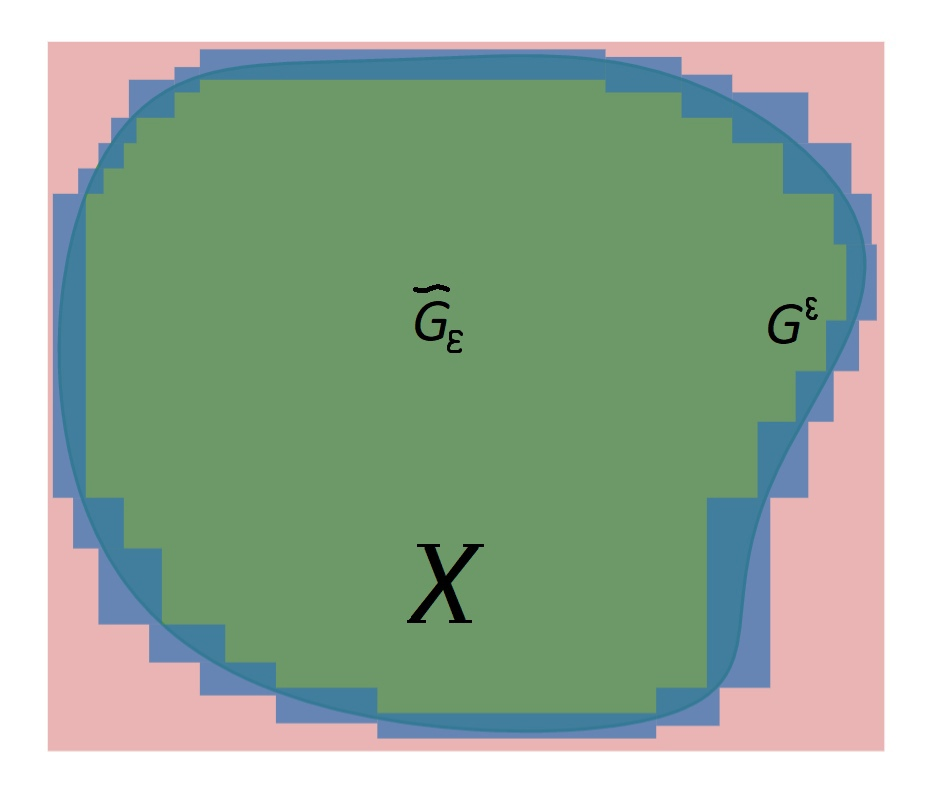
\includegraphics[scale=0.25]{Q(Клет).jpg}
\end{wrapfigure}

\noindent Тогда есть два варианта:

\noindent $\left[Q_j \subset X\right]$ либо $\left[Q_j \cap X = \varnothing\right]$

\vspace{2mm}

\noindent Пусть без потери общности $Q_1, Q_2, \ldots, Q_l$: $\text{} Q_j \subset X$, $j = \overline{1,l}$;

\noindent $Q_{l+1}, Q_{l+2}, \ldots, Q_k:\text{ } Q_j \cap X = \varnothing$, $j = \overline{l+1,k}$;


\begin{equation*}
	\widetilde{G_{\varepsilon}} = \bigcup\limits_{j = 1}^l Q_j, \hspace{5mm} \widetilde{G^{\varepsilon}} = \widetilde{G_{\varepsilon}} \cup G^{\varepsilon} = Q \backslash \left(\bigcup\limits_{j = l + 1}^k Q_j\right)
\end{equation*}


\noindent $\widetilde{G_{\varepsilon}} \subset X \subset \widetilde{G^{\varepsilon}}$

\noindent $m(G^{\varepsilon}) = m(\widetilde{G^{\varepsilon}}) - m(\widetilde{G_{\varepsilon}}) < \varepsilon \Rightarrow$ $X$ измеримо по Жордану.

\subsection*{Примеры неизмеримых по Жордану множеств}

\noindent \boxed{1} $X = \{x \in [0, 1]: x \in \mathbb{Q}\}, \text{ }X \subset \mathbb{E}^1$.

$\partial X = [0,1] \Rightarrow m(\partial X) = 1 \neq 0$ $\Rightarrow X$ неизмеримо.

\vspace{5mm}
\noindent \boxed{2} $Y = X\times X$, где $X$ из \boxed{1}.

$\partial Y = [0,1]\times [0,1] \Rightarrow$ $m(\partial Y) = 1 \neq 0$ $\Rightarrow Y$ неизмеримо.

\vspace{5mm}
\noindent \boxed{3} $X$ из \boxed{1}. $X = \{a_1, a_2, \ldots, a_n, \ldots\}$, $0 \leqslant a_j \leqslant 1$

Пусть $B = \bigcup\limits_{j = 1}^{\infty} \left(a_j - \frac{\varepsilon}{2^j}; a_j + \frac{\varepsilon}{2^j}\right)$, $0 < \varepsilon < \frac{1}{2}$.

$B$ открыто как объединение открытых множеств.

Обозначим $B_k = \bigcup\limits_{j = 1}^k \left(a_j - \frac{\varepsilon}{2^j}; a_j + \frac{\varepsilon}{2^j}\right)$


$m(B_k) \leqslant \sum\limits_{j = 1}^k \frac{\varepsilon}{2^{j-1}} = \varepsilon \left(\frac{1}{2} + \frac{1}{4} + \ldots + \frac{1}{2^{k-1}}\right) = \varepsilon \frac{1 - \frac{1}{2^k}}{\frac{1}{2}} = 2\varepsilon \left(1 - \frac{1}{2^k}\right) < 2\varepsilon$

Тогда $\underline{m}(B) \leqslant 2\varepsilon < 1$. Но $[0, 1]\subset B \Rightarrow \overline{m}(B) > 1$.

То есть $\underline{m}(B) \neq \overline{m}(B) \Rightarrow$  $B$ неизмеримо.


\subsection*{Измеримость объединения, пересечения и разности измеримых множеств}

$\textbf{1}^\circ$ Если $X_1$ и $X_2$ измеримы по Жордану, то $X_1 \cup X_2$, $X_1 \cap X_2$, $X_1 \backslash X_2$ - измеримые по Жордану множества.

\noindent \textbf{Доказательство:}

$X_1$ и $X_2$ измеримы по Жордану $\Rightarrow$ $X_1$ и $X_2$ ограничены и $m(\partial X_1) = m(\partial X_2) = 0$. Тогда и $m(\partial X_1 \cup \partial X_2) = 0$.
\vspace{3mm}

\noindent $\underbrace{\partial (X_1 \cup X_2) \subset \partial X_1 \cup \partial X_2;\text{ } \partial (X_1 \cap X_2) \subset \partial X_1 \cup \partial X_2;\text{ } \partial (X_1 \backslash X_2) \subset \partial X_1 \cup \partial X_2}_{\Downarrow}$	

$m(\partial (X_1 \cup X_2)) = m(\partial (X_1 \cap X_2)) = m(\partial (X_1 \backslash X_2)) = 0 \Rightarrow$

\vspace{2mm}
\noindent $\Rightarrow X_1 \cup X_2, X_1 \cap X_2$ и $ X_1 \backslash X_2$ измеримы.


\subsection*{Конечная аддитивность меры Жордана}

$\textbf{2}^\circ$ Пусть $X_1, X_2, \ldots, X_k$ - измеримые по Жордану множества, тогда множество $X = \bigcup\limits_{j = 1}^k X_j$ измеримо и:

1) $m(X) \leqslant \sum\limits_{j = 1}^k m(X_j)$;

2) Если $X_j \cap X_i = \varnothing$ при $i \neq j$, то $m(X) = \sum\limits_{j = 1}^k m(X_j)$.

\noindent \textbf{Доказательство:} (для $k = 2$, а дальше по индукции)

\vspace{2mm}

1) $X_1$ и $X_2$ измеримы по Жордану $\Rightarrow X = X_1 \cup X_2$ измеримо.

$\forall \varepsilon > 0$ $\exists G_1^{\varepsilon}, G_2^{\varepsilon}$: $X_1 \subset G_1^{\varepsilon}$, $X_2 \subset G_2^{\varepsilon}$ и: 

$m(X_1) > m(G_1^{\varepsilon}) - \frac{\varepsilon}{2}$

$m(X_2) > m(G_2^{\varepsilon}) - \frac{\varepsilon}{2}$

\vspace{2mm}

Тогда $G^{\varepsilon} = G_1^{\varepsilon} \cup G_2^{\varepsilon}$ - клеточное множество и $X \subset G^{\varepsilon}$.

Получаем:

$m(X) \leqslant m(G^{\varepsilon}) \leqslant m(G_1^{\varepsilon}) + m(G_2^{\varepsilon}) < m(X_1) + m(X_2) + \varepsilon$.

\vspace{2mm}

В силу произвольности $\varepsilon \Rightarrow$ $m(X) \leqslant m(X_1) + m(X_2) \hspace{42mm} \boxed{*}$

\vspace{5mm}
2) $X_1 \cap X_2 = \varnothing$, $X = X_1 \cup X_2$

$\forall \varepsilon > 0$ $\exists G_{\varepsilon}^1, G_{\varepsilon}^2$: $G_{\varepsilon}^1 \subset X_1$, $G_{\varepsilon}^2 \subset X_2$ и:

$m(G_{\varepsilon}^1) > m(X_1) - \frac{\varepsilon}{2}$

$m(G_{\varepsilon}^2) > m(X_2) - \frac{\varepsilon}{2}$

\vspace{2mm}

$G_{\varepsilon} = G_{\varepsilon}^1 \cup G_{\varepsilon}^2$ и $G_{\varepsilon}^1 \cap G_{\varepsilon}^2 = \varnothing$, а также $G_{\varepsilon}^1 \cup G_{\varepsilon}^2 \subset X$.

\vspace{2mm}

Тогда $m(X) \geqslant m(G_{\varepsilon}) = m(G_{\varepsilon}^1) + m(G_{\varepsilon}^2) > m(X_1) + m(X_2) - \varepsilon$.

\vspace{2mm}

В силу произвольности $\varepsilon > 0$ получаем $m(X) \geqslant m(X_1) + m(X_2) \hspace{16mm} \boxed{**}$ 

\vspace{2mm}

Из $\boxed{*}$ и $\boxed{**}$ $\Rightarrow$ $m(X) = m(X_1) + m(X_2)$

\subsection*{Измеримость и мера цилиндра в (m+1)-мерном пространстве}

\noindent \textbf{Предложение:} пусть $X \subset \mathbb{E}^m$, $m \geqslant 1$, - измеримо, тогда множество $Y = X\times [a, b) \subset \mathbb{E}^{m + 1}$ - измеримо. $m(Y) = m(X)(b - a)$.

\noindent \textbf{Доказательство:}

\noindent $\left[X \text{ измеримо}\right] \stackrel{\text{def}}{=} \left[\forall \varepsilon > 0\text{ }\exists G_{\varepsilon}, G^{\varepsilon}: G_{\varepsilon}\subset X\subset G^{\varepsilon}, \text{ } m(G^{\varepsilon}) - m(G_{\varepsilon}) < \frac{\varepsilon}{b - a}\right]$.

\vspace{2mm}

\noindent Рассмотрим клеточные множества:

\noindent $\widetilde{G_{\varepsilon}} = G_{\varepsilon}\times [a, b)$ и $\widetilde{G^{\varepsilon}} = G^{\varepsilon}\times [a, b)$;

\vspace{2mm}

\noindent Тогда $\widetilde{G_{\varepsilon}} \subset Y \subset \widetilde{G^{\varepsilon}}$, а $m(\widetilde{G_{\varepsilon}}) = m(G_{\varepsilon})(b-a)$ и $m(\widetilde{G^{\varepsilon}}) = m(G^{\varepsilon})(b-a)$;

\noindent Получаем:

\noindent $m(\widetilde{G^{\varepsilon}}) - m(\widetilde{G_{\varepsilon}}) = (m(G^{\varepsilon}) - m(G_{\varepsilon}))(b-a) < \frac{\varepsilon}{b-a}(b-a) = \varepsilon$ $\Rightarrow Y$ измеримо.

	
\end{document}